% -*- TeX:de -*-
\NeedsTeXFormat{LaTeX2e}
\documentclass[12pt,a4paper]{article}
\usepackage[german]{babel} % german text
\usepackage[DIV12]{typearea} % size of printable area
\usepackage[T1]{fontenc} % font encoding
%\usepackage[latin1]{inputenc} % most likely on Windows
\usepackage[utf8]{inputenc} % probably on Linux
\usepackage{multicol}

% PLOTTING
\usepackage{pgfplots} 
\usepackage{pgfplotstable}
\usepackage{url}
\usepackage{graphicx} % to include images
\usepackage{tikz}
\usepackage{subfigure} % for creating subfigures
\usepackage{amsmath} % a bunch of symbols
\usepackage{amssymb} % even more symbols
\usepackage{booktabs} % pretty tables
\usepackage{makecell} % multi row table heading

% a floating environment for circuits
\usepackage{float}
\usepackage{caption}

%\newfloat{circuit}{tbph}{circuits}
%\floatname{circuit}{Schaltplan}

% a floating environment for diagrams
%\newfloat{diagram}{tbph}{diagrams}
%\floatname{diagram}{Diagramm}

\selectlanguage{german} % use german

\begin{document}

%%%%%%% DECKBLATT %%%%%%%
\thispagestyle{empty}
			\begin{center}
			\Large{Fakultät für Physik}\\
			\end{center}
\begin{verbatim}


\end{verbatim}
							%Eintrag des Wintersemesters
			\begin{center}
			\textbf{\LARGE SS 14}
			\end{center}
\begin{verbatim}


\end{verbatim}
			\begin{center}
			\textbf{\LARGE{Physikalisches Praktikum\\ für das Bachelorstudium}}
			\end{center}
\begin{verbatim}




\end{verbatim}

			\begin{center}
			\textbf{\LARGE{PROTOKOLL}}
			\end{center}
			
\begin{verbatim}

\end{verbatim}

			\begin{flushleft}
			\textbf{\Large{Experiment (Nr., Titel):}}\\
							%Experiment Nr. und Titel statt den Punkten eintragen
			\LARGE{PS06 Strahlung}	
			\end{flushleft}

\begin{verbatim}

\end{verbatim}	
							%Eintragen des Abgabedatums, oder des Erstelldatums des Protokolls
			\begin{flushleft}
			\textbf{\Large{Datum:}} \Large{20.3.2014}
			\end{flushleft}
			
\begin{verbatim}
\end{verbatim}
							%Namen der Protokollschreiber
		\begin{flushleft}
			\textbf{\Large{Namen:}} \Large{Patrick Braun, Johannes Kurz}
			\end{flushleft}

\begin{verbatim}


\end{verbatim}
							%Kurstag und Gruppennummer, zb. Fr/5
			\begin{flushleft}
			\textbf{\Large{Kurstag/Gruppe:}} \Large{DO/4}
			\end{flushleft}

\begin{verbatim}

\end{verbatim}
							%Name des Betreuers, das Praktikum betreute.
			\begin{flushleft}
			\LARGE{\textbf{Betreuer:}}	\Large{Erhard Schafler}	
			\end{flushleft}

%%%%%%% DECKBLATT ENDE %%%%%%%
\pagebreak
\setlength{\columnsep}{20pt}
\begin{multicols}{2}

%%%%%%%%%%%%%%%%%%%%%%%%%%%%%%%%%%%%%%%%%%%%%%%%

%\begin{figure}[H]
%	\centering
%	\includegraphics[scale=0.35]{./data/beugung.png}
%	\caption{Beugungsmuster Einzelspalt (echtes Foto; schwarz durch weiß ersetzt)}
%	\label{fig:beugungsmuster}
%\end{figure}


%\begin{figure}[H]
%	\centering
%	\pgfplotstabletypeset[
%			columns={abstand, n},
%			col sep=&,
%			columns/abstand/.style={precision=2, zerofill, column name=\makecell{$Abstand$\\$(\pm 0.05)[mm]$} }, 
%			columns/n/.style={column name=\makecell{$n$\\$(Ordnung)$}, precision=0},
%			every head row/.style={before row=\hline,after row=\hline\hline},
%			every last row/.style={after row=\hline},
%			every first column/.style={column type/.add={|}{} },
%			every last column/.style={column type/.add={}{|} }
%			]{
%			abstand & n
%			12.9 & 1
%			24.45 & 2
%			37.40 & 3
%			49.35& 4
%			62.45 & 5
%			74.45 & 6
%			87.45 & 7
%			100.25 & 8
%			
%			}
%	\caption{Messwerte Einzelspalt}
%	\label{tab:werte_einzelspalt}
%\end{figure}



%%%%%%%%%%%%%%%%%%%%%%%%%%%%%%%%%%%%%%%%%%%%%%%%
%%%%%%%%%%%%%%%%%%%%%%%%%%%%%%%%%%%%%%%%%%%%%%%%
\section{Planck'sches Wirkungsquantum}

\subsection{Grundlagen, Theorie und Versuchsaufbau}

In diesem Versuch wird das Plank'sche Wirkungsquantum unter Zuhilfenahme des Fotoelektrischen Effekt bestimmt.\\
Der Zusammenhang
$$E = h * \nu$$
E \ldots Energie \\
h \ldots Plankkonstante \\ 
$\nu$ \ldots Frequenz \\
\\
Basierend auf dem fotoelektrischen Effekt wird durch Einstrahlung von Licht einer bestimmten Frequenz aus einem Materiel ein Ladungsträger (Elektron) angeregt [1](p. 3) und vom Valenzband in das Leitungsband angehoben. Zusätzlich erhalten die Elektronen kinetische Energie.\\
Einstein stellte den Zusammenhang wie folgt dar:
$$U_0(\nu) = \frac{h}{e} * \nu - \frac{A}{e}$$
$U_0$ \ldots Gegenspannung\\
e \ldots Elementarladung\\
A \ldots Austrittsarbeit\\

\noindent 
Der Aufbau des Versuches ist in \ref{fig:Plank_Aufbau} ersichtlich. Dabei wird Licht durch einen Filter auf einen Wellenlängenbereich begrenzt und auf ein Kathode im Vakuum gesendet. Hierbei werden Elektronen gelöst und zur Anode (links) geschleudert. Dabei muss die aufgenommene Energie die Austrittsarbeit überschreiten [1](p. 3-4).\\
Auf Anodenseite kann der Fotostrom und auf Kathodenseite die angebrachte Gegenspannung gemessen werden.

\begin{figure}[H]
	\centering
	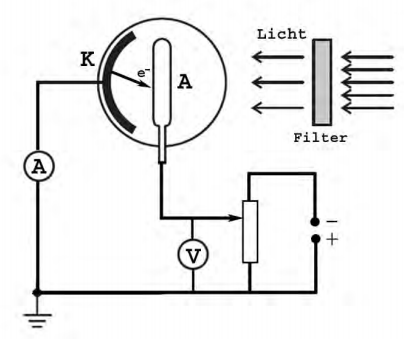
\includegraphics[scale=0.5]{./data/Planck_Aufbau.png}
	\caption{Aufbau der Gegenfeld-Kompensationsmethode [1](p. 4, Abbildung 2)}
	\label{fig:Plank_Aufbau}
\end{figure}

\noindent 
Trägt man bei mehreren Frequenzen (Filtern) den Fotostrom gegen die Gegenspannung auf, bestimmt den Achsenabschnitt einer linearen Regression der Anfangssteigung (Gefälle) so erhält man frequenzabhängige Werte für $U_0$. 
Der resultierende Graph lässt sich beschreiben wie eine Geradengleichung (U = k * x + d, vergleiche Einstein'sche Gleichung oben).\\
Die Steigung ergibt das Wirkungsquantum. Der Achsenabschnitt (Abszisse) entspricht der Arbeit die geleistet werden muss um ein Elektron vom Material zu lösen. \\
Die Auswertung, Regressionen und Berechnungen werden im folgenden Punkt aufgeführt.

\end{multicols}
\subsection{Resultate}


\begin{figure}[H]
	\centering
	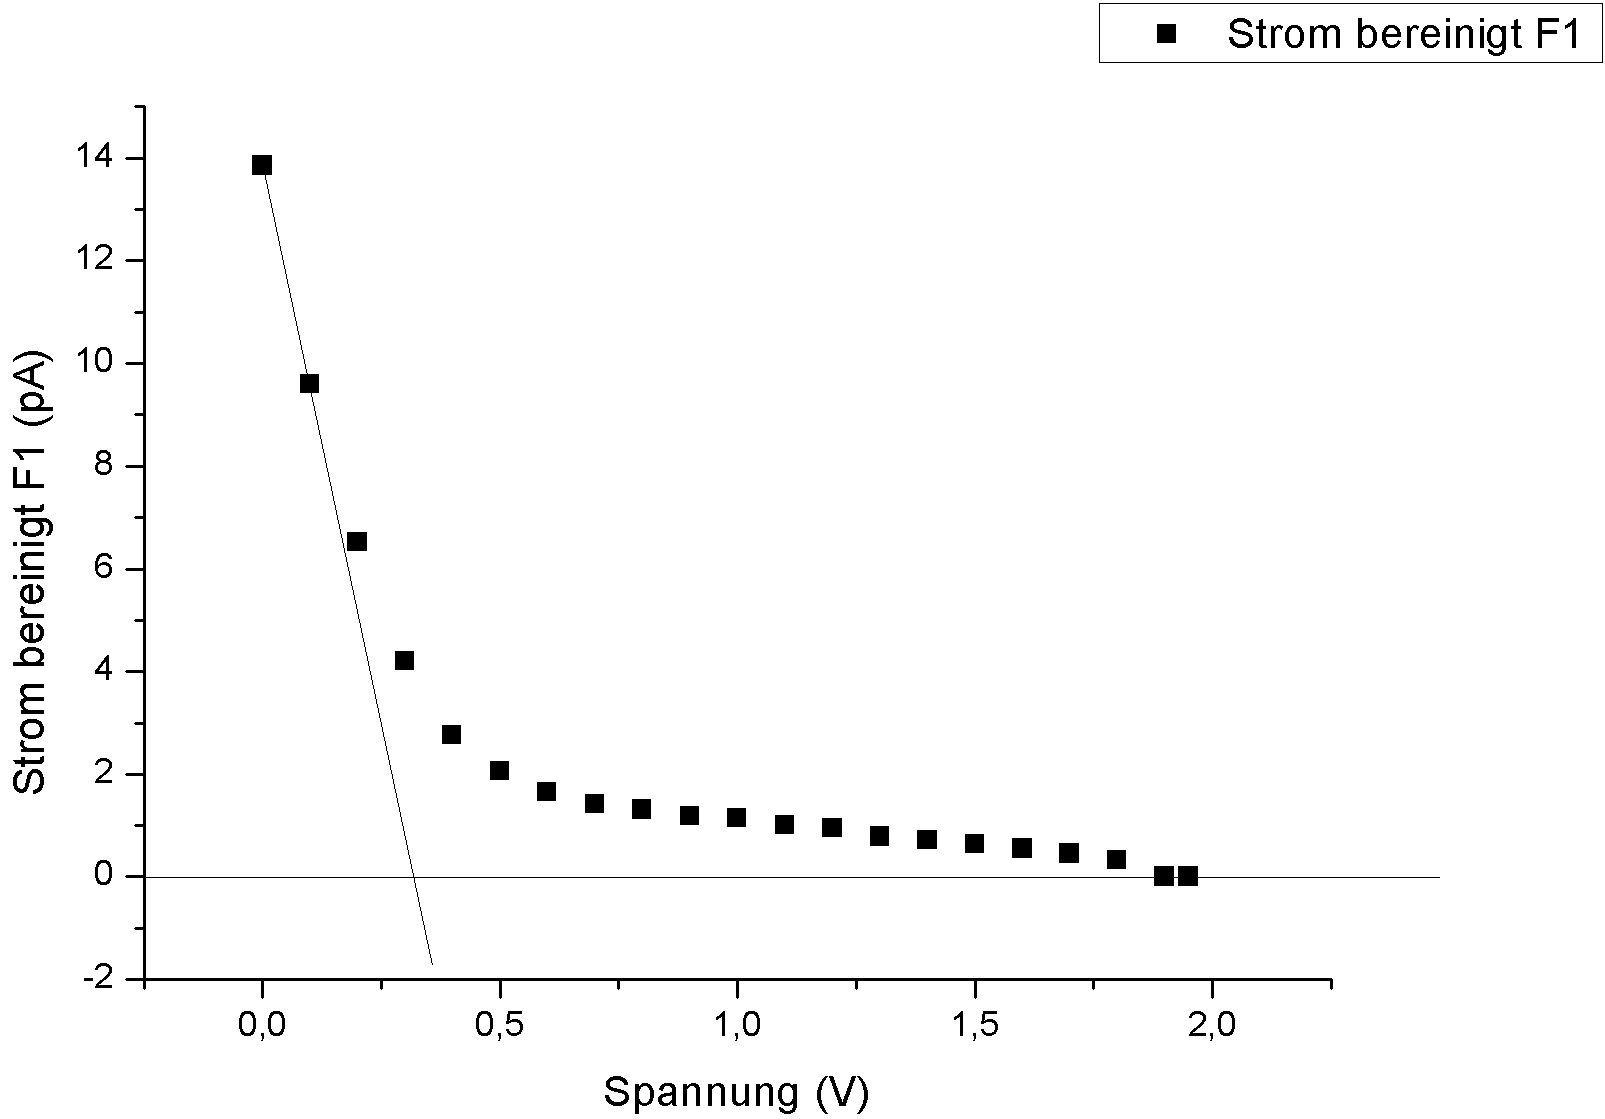
\includegraphics[scale=0.5]{./data/Filter1.png}
	\caption{Intensitäten (Spannungen) mit 1. Filter}
	\label{fig:filter1}
\end{figure}

\begin{figure}[H]
	\centering
	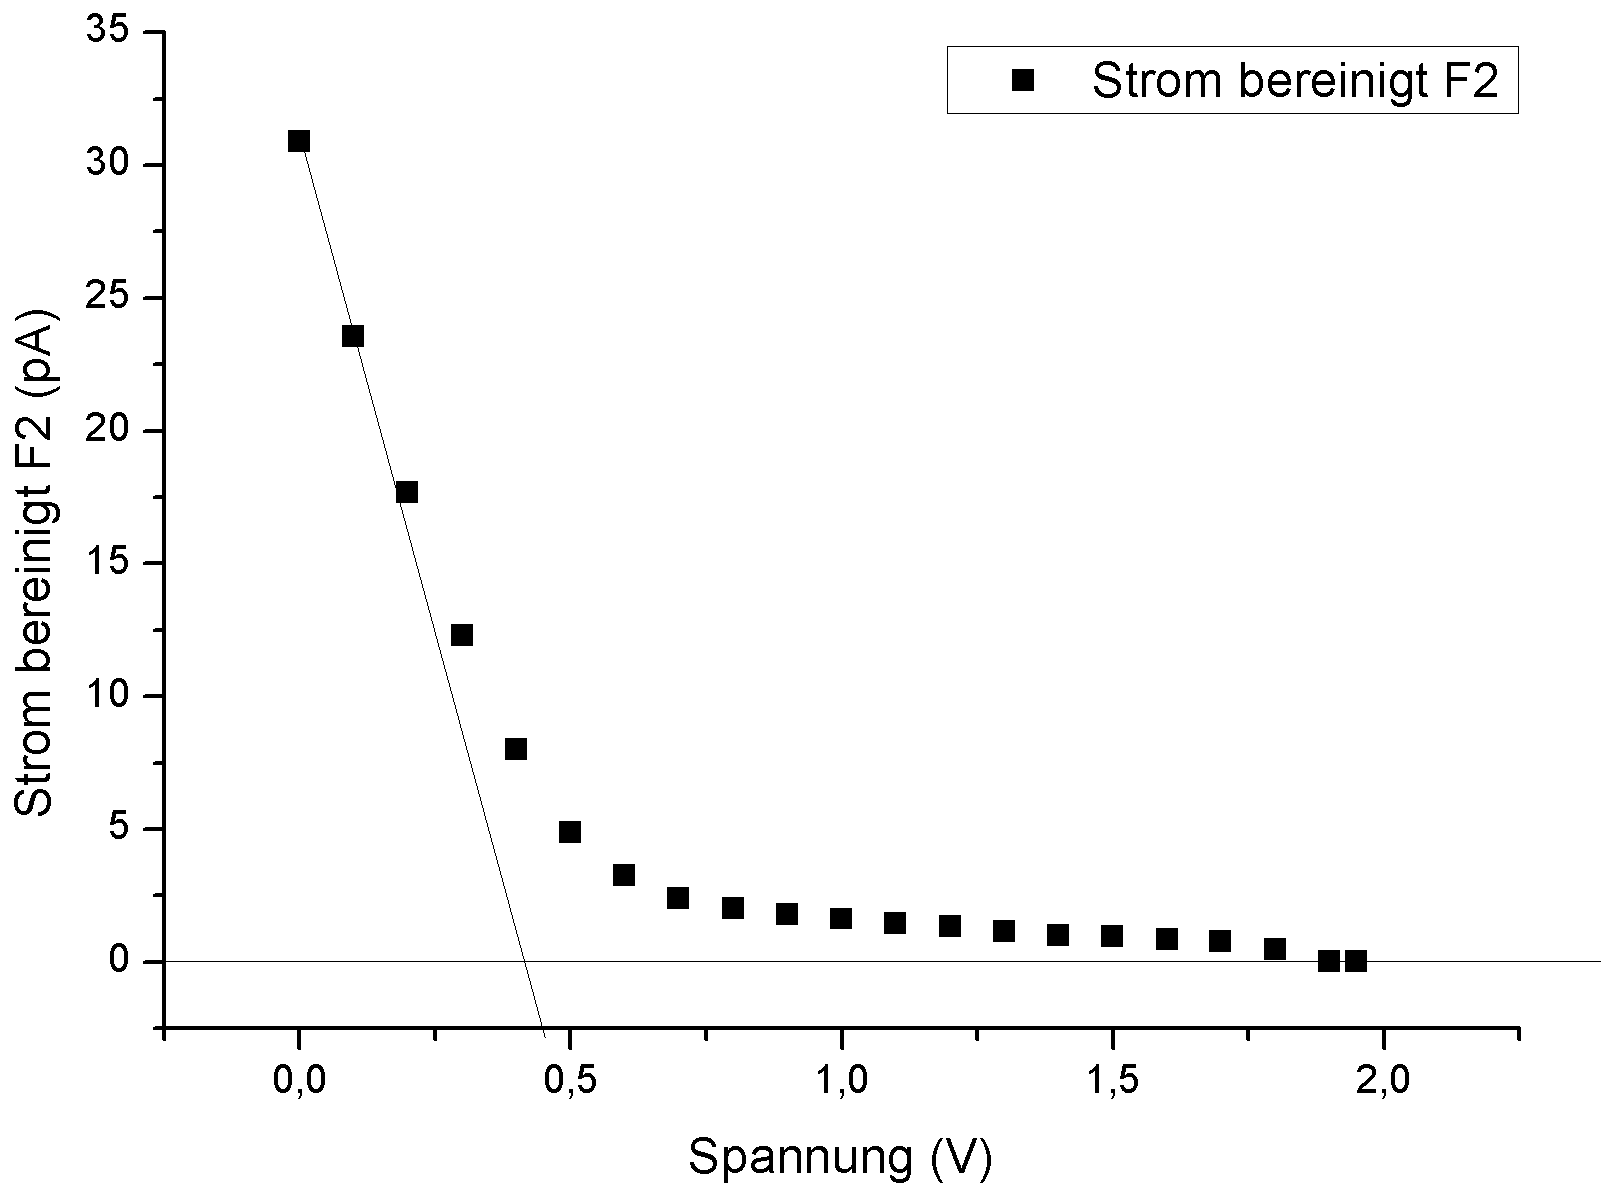
\includegraphics[scale=0.5]{./data/Filter2.png}
	\caption{Intensitäten (Spannungen) mit 2. Filter}
	\label{fig:filter2}
\end{figure}

\begin{figure}[H]
	\centering
	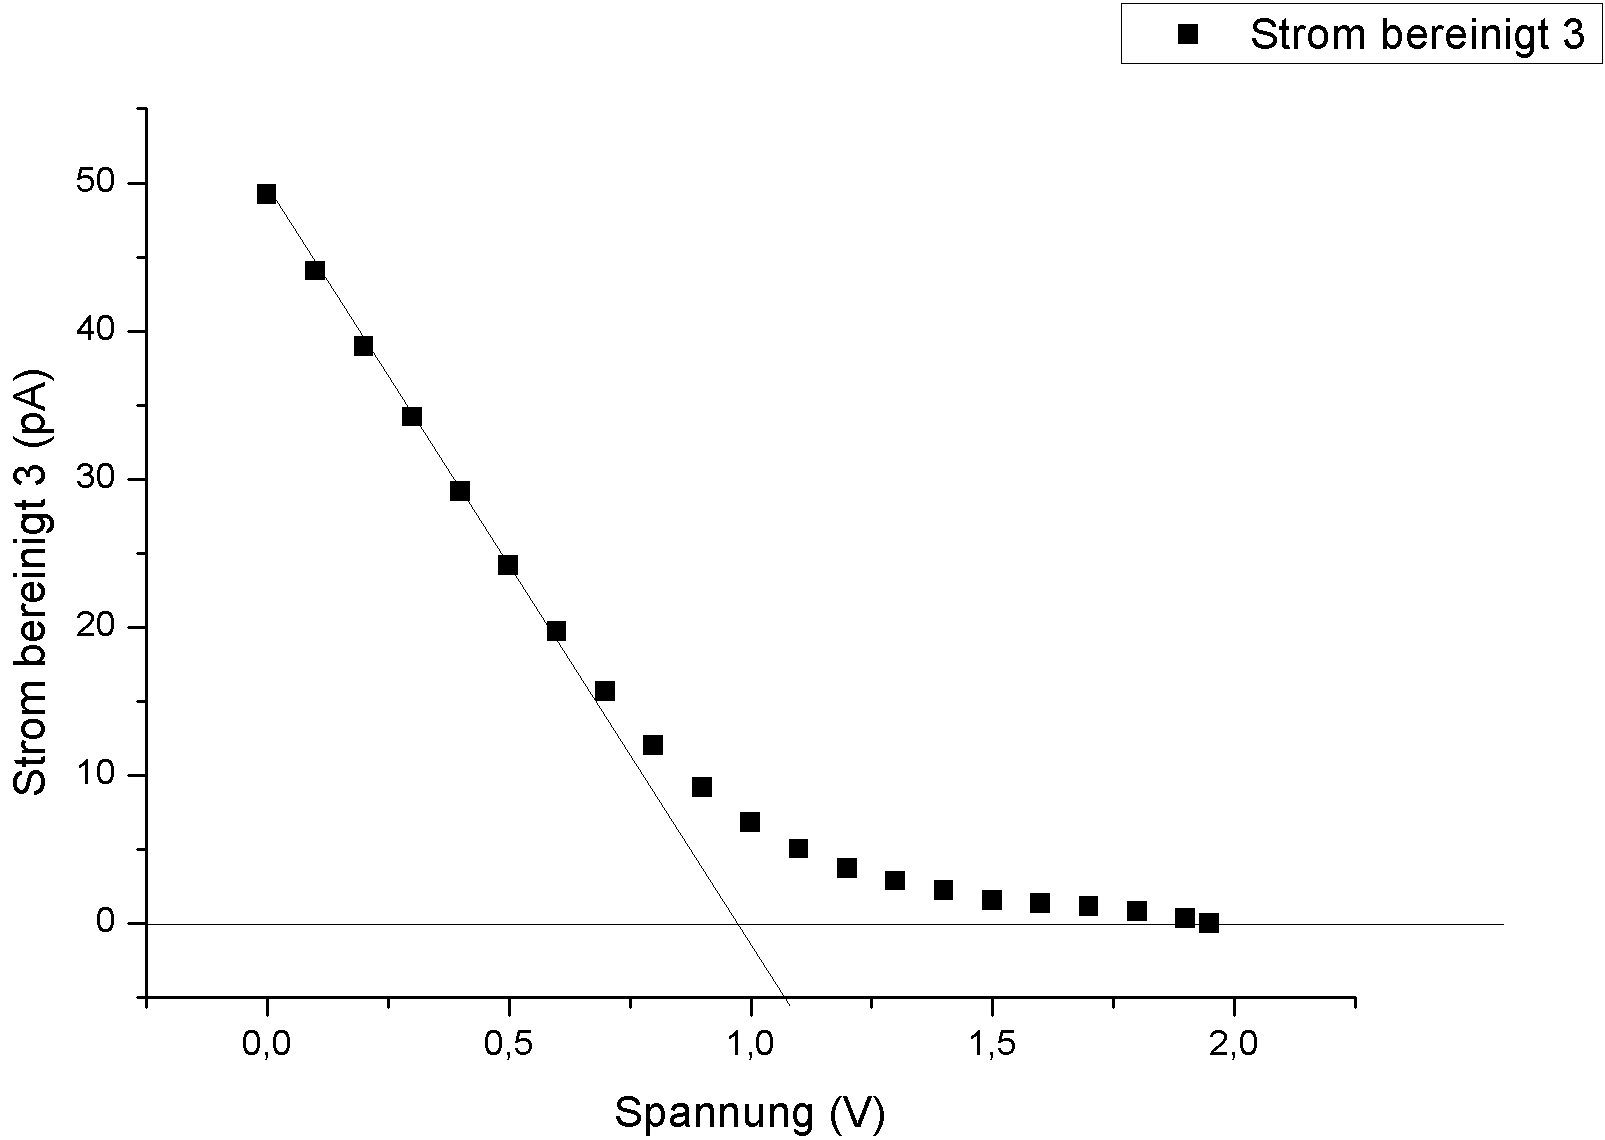
\includegraphics[scale=0.5]{./data/Filter3.png}
	\caption{Intensitäten (Spannungen) mit 3. Filter}
	\label{fig:filter3}
\end{figure}

\begin{figure}[H]
	\centering
	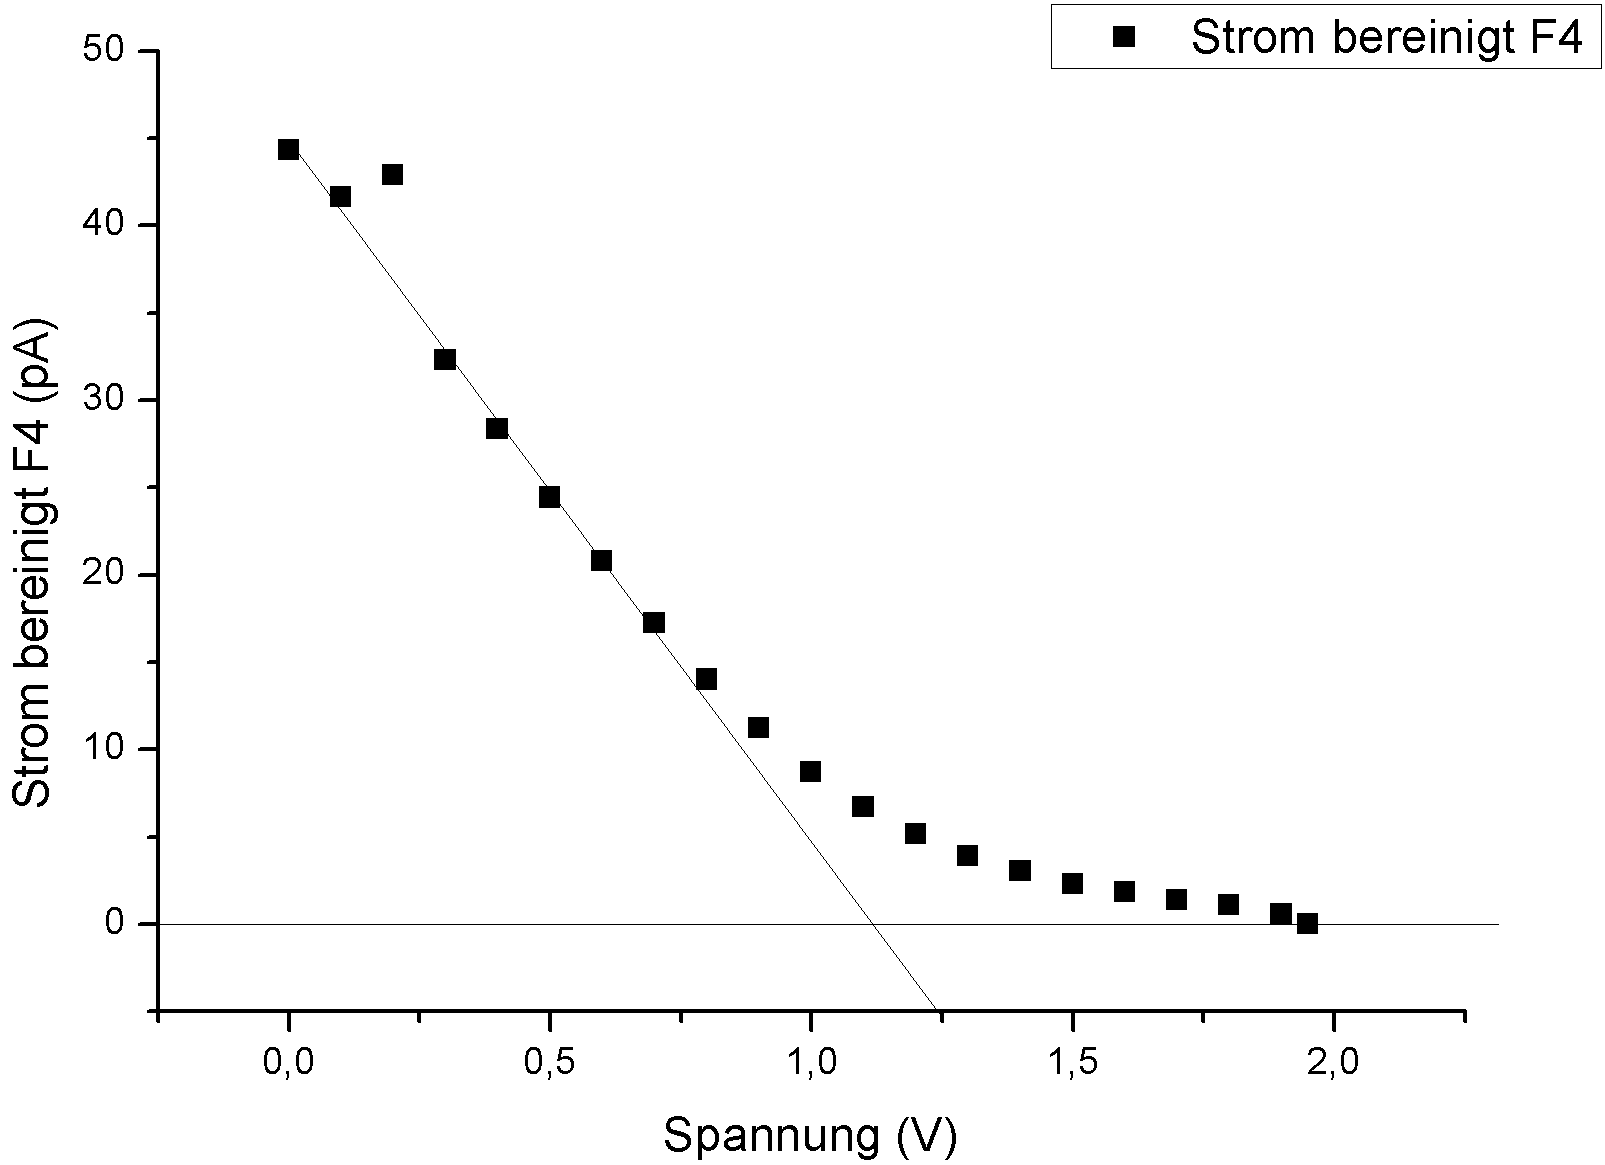
\includegraphics[scale=0.5]{./data/Filter4.png}
	\caption{Intensitäten (Spannungen) mit 4. Filter}
	\label{fig:filter4}
\end{figure}

\begin{figure}[H]
	\centering
	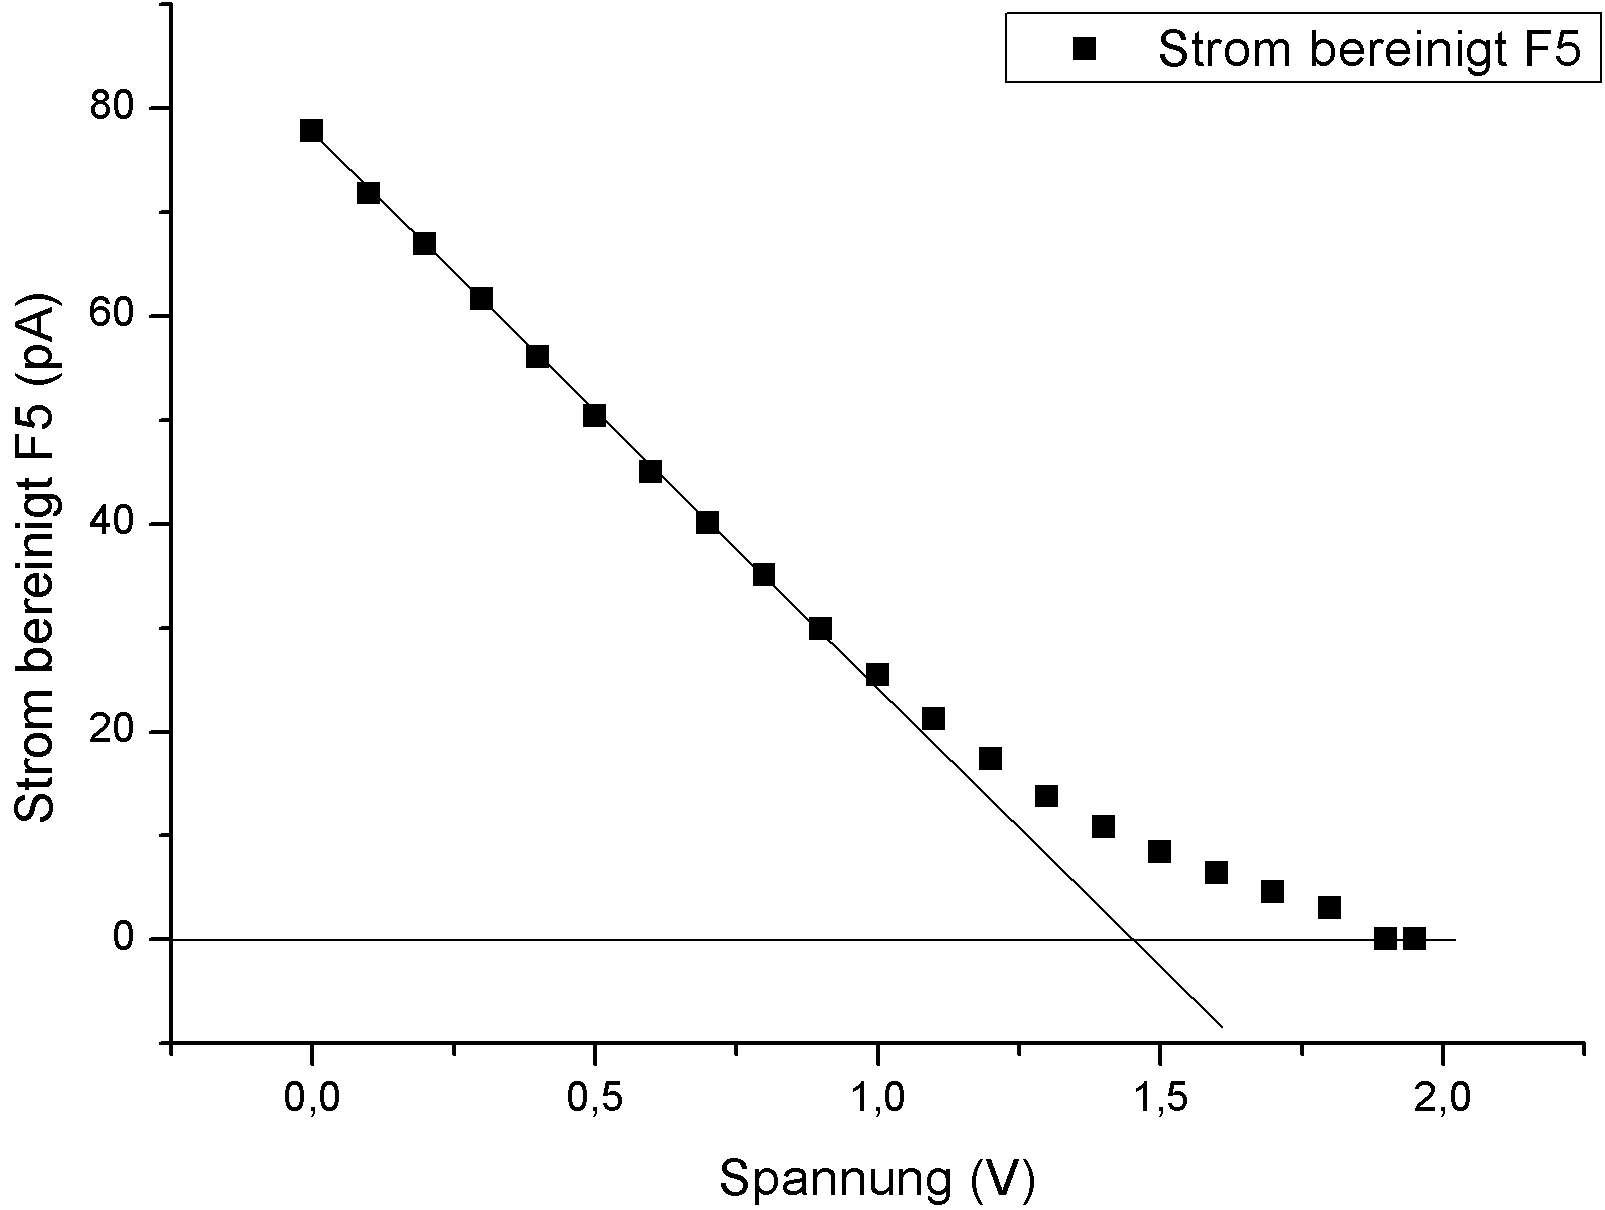
\includegraphics[scale=0.5]{./data/Filter5.png}
	\caption{Intensitäten (Spannungen) mit 5. Filter}
	\label{fig:filter5}
\end{figure}

\begin{figure}[H]
	\centering
	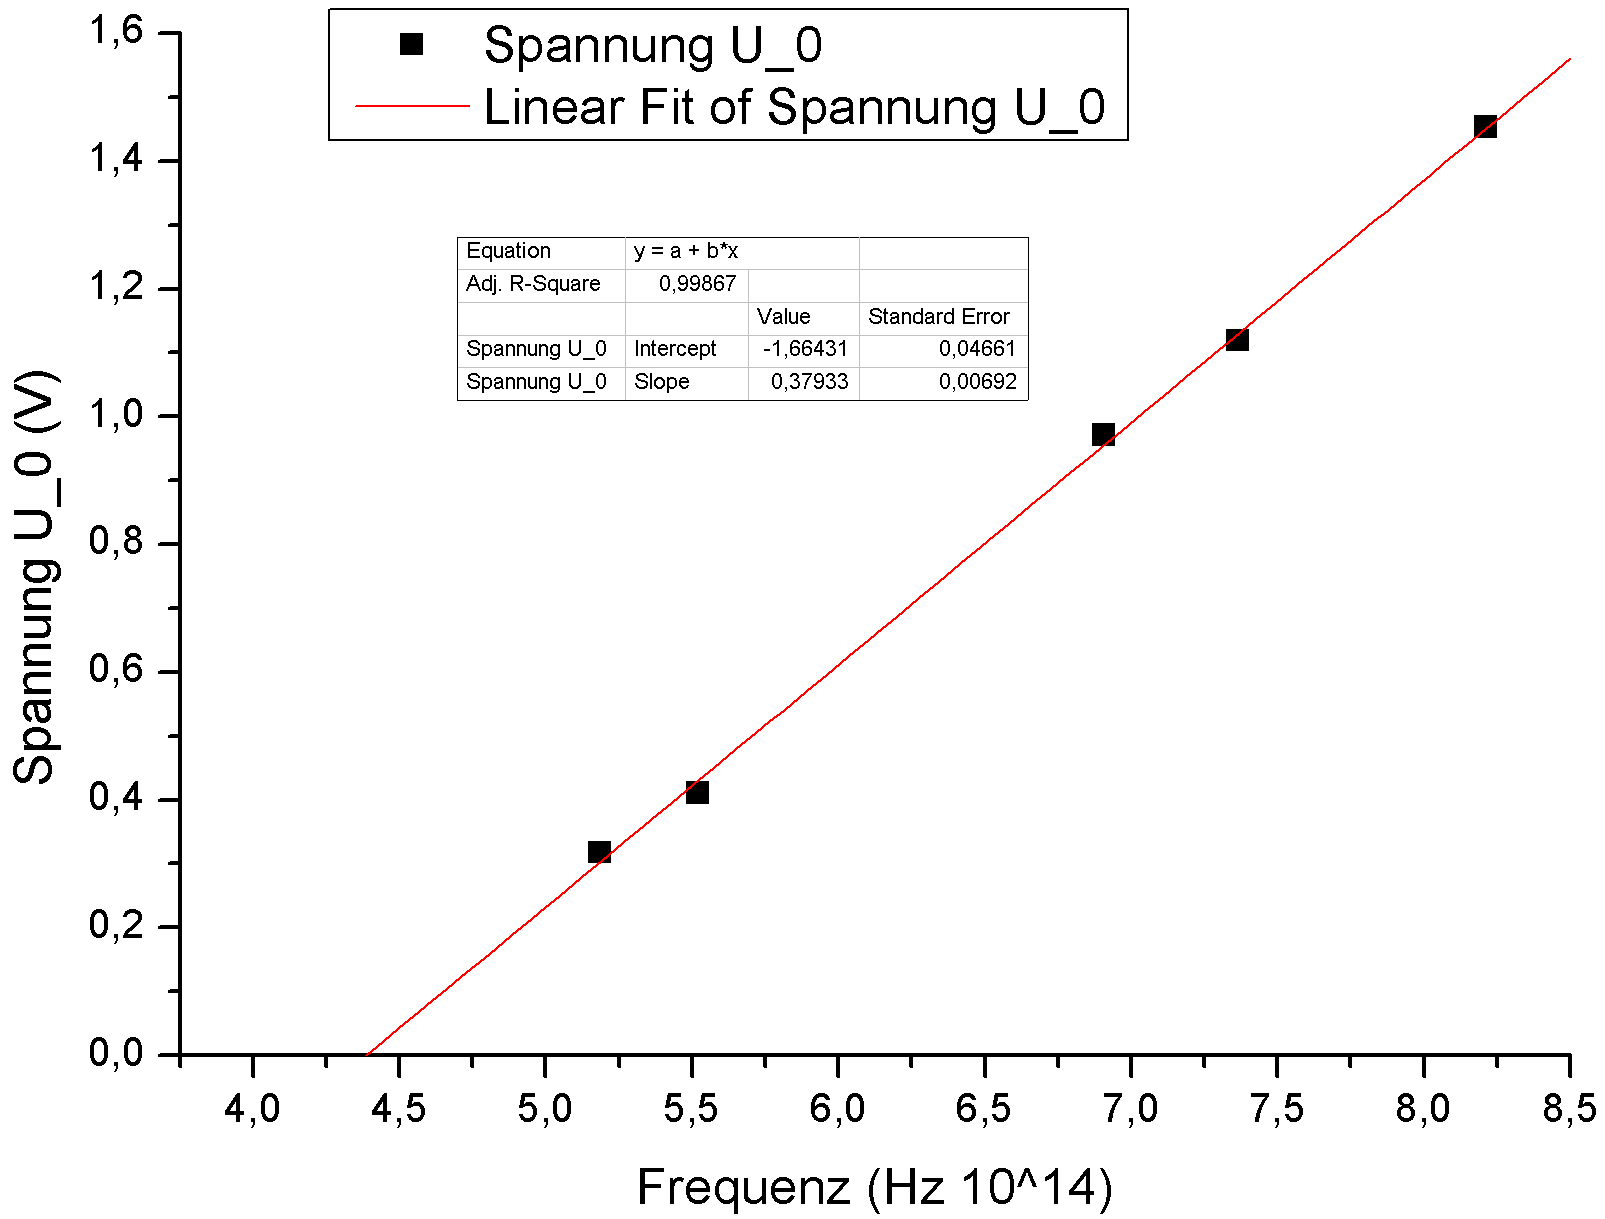
\includegraphics[scale=0.45]{./data/U0_Plank.png}
	\caption{Spannungen gegen Frequenz}
	\label{fig:plank}
\end{figure}
\begin{multicols}{2}


\noindent $$h=(6.08 \pm 0.12)\times 10^{-34} m^2kg/s$$
$$A=(1.664\pm 0.047)eV$$
$$\nu_g=(4.35\pm 0.05)\times 10^{14} Hz$$



\subsection{Diskussion}

Die Methode, die, trotz hochauflösendem Amperemeter und Fotozelle, auf makroskopischen und grob wirkenden Mitteln aufbaut, liefert ein erstaunlich genaues Ergebnis für eine so kleine Größe, wie das Planck-Wirkungsquantum. Das Ergebnis liegt in der richtigen Größenordnung und um weniger als 9\% neben dem Literaturwert.\\
Die bestimmte Unsicherheit der Messung (die die Unsicherheit aus dem linearen Fit ist) covert diesen Abstand jedoch nicht.\\
Abgesehen von der Messung selbst, der Qualität der Apparatur und anderen äußeren EInflüssen, spielt vermutlich vor allem das Abschätzen der Geraden in den einzelnen Messungen eine Rolle.\\
Dieses wurde "von Hand" geschätzt, da diese Methode genauer scheint, als einen Fit durch einen bestimmten Bereich der Kurven zu legen. Schließlich weisen diese schon früh eine Krümmung auf.\\
Dadurch spielt auch der Ausreißer im 4. Filter (Abb.\ref{fig:filter4}) keine Rolle, da er im Fitting ignoriert wurde.\\
Trotzdem kann der restliche (erwartungsgemäße) Verlauf der Kurve  keine Begründung für den Ausreißer sein; auf das Ziel dieses Versuches dürfte er jedoch keinen Einfluss haben. Ein Vergleich mit den Messungen der anderen Gruppen würde zeigen, ob dieser Wertesprung immer auftritt, oder einzigartig war.\\



%%%%%%%%%%%%%%%%%%%%%%%%%%%%%%%%%%%%%%%%%%%%%%%%
%%%%%%%%%%%%%%%%%%%%%%%%%%%%%%%%%%%%%%%%%%%%%%%%
\section{Wärmestrahlung}

In diesem Versuch wird die Temperatur des Glühdrahtes einer Glühbirne gemessen, unter Ausnutzung der Wärmestrahlung, die von ihm abgegeben wird.

\subsection{Grundlagen, Theorie und Versuchsaufbau}

Jeder Körper emittiert Wärmestrahlung. Ab einer gewissen Temperatur kommt auch sichtbares Licht dazu (wie eben in einer Glühbirne).\\

\textbf{Aufbau:}\\
Die Glühlampe, ein Filter und eine Fotozelle (zur Messung der Intentsität) sind auf einer Schiene montiert. Strom sowie Spannung, mit der die Glühbirne versorgt wird, werden mit 2 Multimetern gemessen (um letztendlich die Leistung zu berechnen); ein weiteres Voltmeter misst die Spannung, nachdem ein Strom-Spannungs-Wandler den Output der Fotozelle übersetzt hat (Abb. \ref{fig:waermestrahlung_aufbau}).




\end{multicols}
\begin{figure}[H]
	\centering
	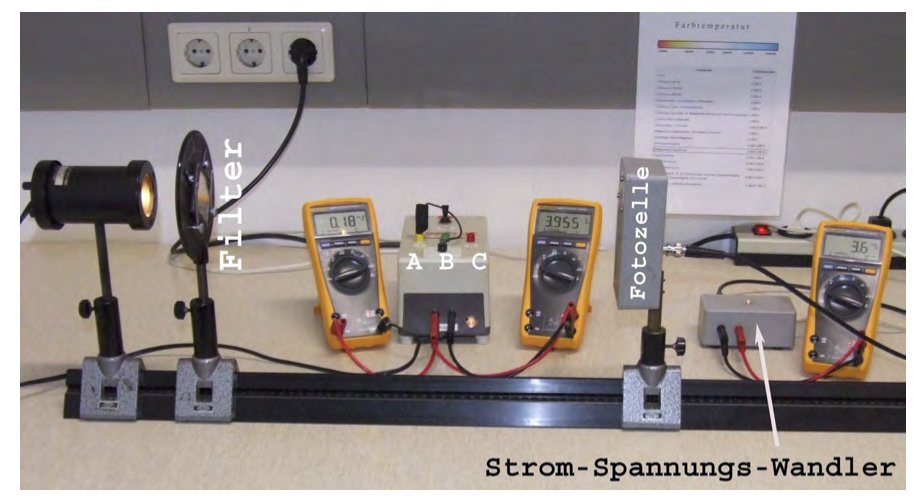
\includegraphics[scale=0.9]{./data/waermestrahlung_aufbau.png}
	\caption{Versuchsaufbau zur Messung der Wärmestrahlung einer Glühlampe}
	\label{fig:waermestrahlung_aufbau}
\end{figure}
\begin{multicols}{2}


Das Licht wird gefiltert um monochromatisches bzw. einen sehr eng eingegrenzten Wellenlängenbereich zu messen (hier $\lambda = 560nm)$. In diesem Versuch wird nämlich das Planck'sche Strahlungsgesetz verwendet, das die Strahlungsenergie, abhängig von Temperatur des strahlenden Körpers und Wellenlänge der Strahlung, angibt:
$$L(\lambda,T)\cdot d \lambda = \frac{2hc^2}{\lambda ^5}\cdot \frac{1}{exp(\frac{hc}{\lambda k T})-1}\cdot d\lambda$$
Verglichen werden im Versuch 2 vorgegebene Einstellungen an der Glühbirne; der Filter bleibt gleich und damit auch die Wellenlänge; Im Quotienten aus beiden Strahlungsformeln ergibt sich, bei gleicher Wellenlänge, dass die Energien im Verhältnis der Intensitäten stehen:
$$\frac{L(\lambda, T_1)}{L(\lambda, T_2)}=\frac{I_1}{I_2}=\frac{exp(\frac{ch}{k\lambda T_2})}{exp(\frac{ch}{k \lambda T_1})}$$

Durch logarithmieren erhält man:

$$ln(\frac{I_1}{I_2})=(\frac{1}{T_2}-\frac{1}{T_1})\cdot \frac{ch}{k\lambda}$$

Weiters wird das Stefan-Boltzmann-Gesetz von der Umwandlung von elektrischer Leistung in Wärme verwendet, um (wiederum im Quotienten beider Konfigurationen) eine Temperatur zu substituieren:

$$\frac{P_1}{P_2}=\frac{T_1^4}{T_2^4}$$

Dieses Verhältnis wird auch benutzt, um, nach Berechnung einer Temperatur, die zweite zu erhalten.\\
Eingesetzt ergibt sich zur Berechnung von $T_1$:
$$T_1=\frac{1}{ln(\frac{I_1}{I_2})}\cdot (\sqrt[4]{\frac{P_1}{P_2}}-1)\cdot \frac{ch}{k\lambda}$$


Die Leistungen $P_1$ und $P_2$ werden durch die gemssenen Ströme und Spannungen berechnet, 
$\lambda$ durch den verwendeten Filter definiert.\\
Um den Quotienten aus den Intensitäten zu erhalten, wird benutzt, dass die Beleuchtungsstärke der Fotozelle durch den Abstand von der Lichtquelle mit $1/r^2$ verringert.\\

Es werden also, für beide Einstellungen an der Lichtquelle, jeweils mehrere Beleuchtungsstärken mit der Fotozelle, für verschiedenen Abständen von der Lichtquelle, gemessen. Diese werden gegen $1/r^2$ aufgetragen, um einen linearen Anstieg zu ergeben. Im linearen Fit beider Daten-Sets erhält man 2 Steigungen, die im gleichen Verhältnis stehen, wie die Intensitäten:
$$\frac{I_1}{I_2}=\frac{r_1^2}{r_2^2}$$.



\end{multicols}
\subsection{Resultate}


\begin{figure}[H]
	\centering
	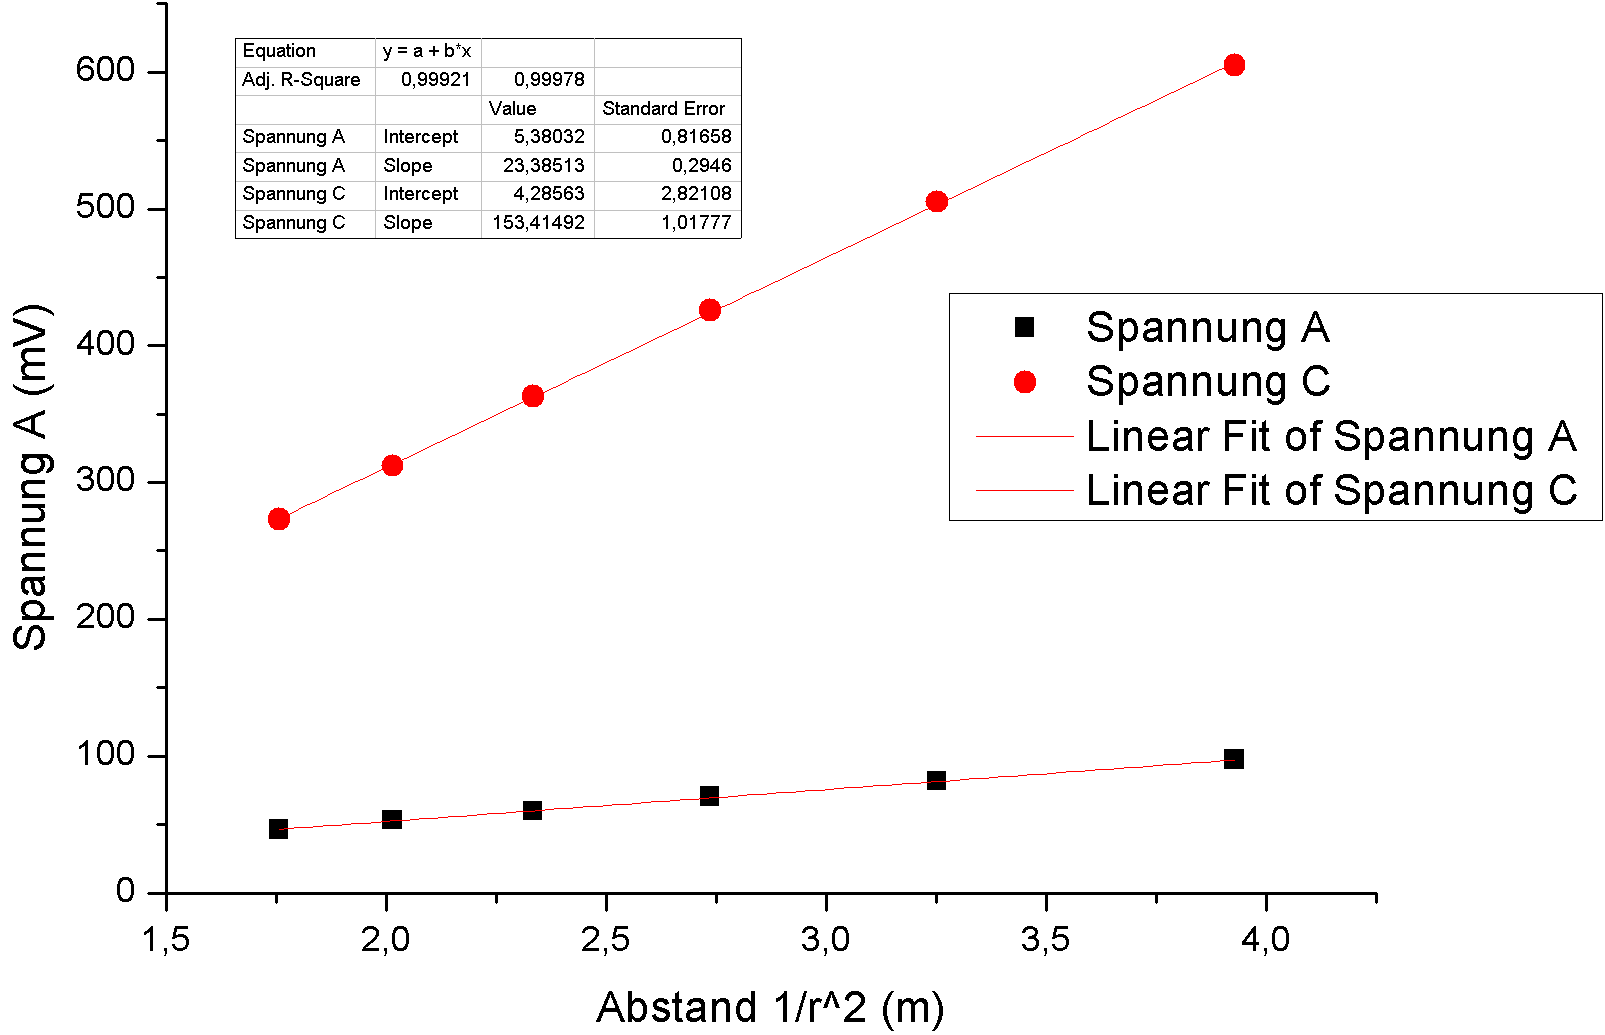
\includegraphics[scale=0.6
	]{data/waermestrahlung.png}
	\caption{Beleuchtungsintensität an der Fotozelle, umgewandelt in Spannung\\
	jeweils 6 verschiedene Abstände}
	\label{fig:waermestrahlung_messung}
\end{figure}
\begin{multicols}{2}

\noindent $\lambda = 560 nm$\\
$P_A$: $I_A=(3.79\pm 0.01)A$\\
\indent $U_A=(3.44\pm 0.01)V$\\
$P_A=(13.038 \pm 0.052)W$\\

\noindent $P_C$: $I_C=(4.82\pm0.01)A$\\
\indent $U_C=(5.45 \pm 0.01)V$\\
$P_C=(26.269 \pm 0.073)W$\\

\noindent $\frac{P_A}{P_C}=(0.4963 \pm 0.0014)$\\

\noindent \textbf{Steigungen:}\\
Konfig A: $r_1^2=(23.39 \pm 0.29)$\\
Konfig B: $r_2^2=(153.4 \pm 1.1)$\\

$\frac{I_A}{I_C}= ( 0.1525 \pm 0.0022)$

$$T_A= (2194\pm 14)K$$
$$T_C=(2613 \pm 17)K$$

\subsection{Diskussion}

$T_A$ wurde aus den gemessenen Werten berechnet, und danach $T_C$ mittels umgeformten Stefan-Boltzmann-Gesetzes.\\
Das Endergebnis ist durch 2 Zwischenergebnisse mit Unsicherheiten behaftet, nämlich durch $\frac{P_A}{P_C}$ und $\frac{I_A}{I_C}$. Dabei kann der Anteil durch das Verhältnis der Beleuchtungsstärken praktisch vernachlässigt werden, da er kleiner als 1K ist, während die Unsicherheit aus dem Verhältnis der Leistungen etwa 13K ausmacht.\\
Um die Messung also noch genauer zu machen, muss vor allem an dieser Stelle angesetzt werden:\\
die Multimeter sind prinzipiell in der Lage genauer zu messen, als von uns angenommen, aufgrund von Fluktuationen jedoch wurde die Unsicherheit auf $0.01A$ bzw. $0.01V$ geschätzt.\\
Nachdem die Messung ausgewertet wurde und die Daten, sowie deren Wirkungen bekannt sind, wäre sicher, bei neuerlicher Messung und wohl bekanntem Verfahren, eine weniger konservative Abschätzung der Messunsicherheit möglich.\\
Außerdem könnte die Messung noch verfeinert werden durch eine stabilere Stromversorgung.\\
Da weder die Schaltung zwischen Modus A und C, noch die Stabilität der Stromversorgung im Versuchsraum, genauer bekannt sind, lässt sich an dieser Stelle darüber keine Aussage treffen.\\

Die sehr grob anmutende Methode, die Fotozelle auf der optischen Schiene zu verrutschen, und im mm-Bereich abzulesen, verursacht jedenfalls, dank linearem Fit, bei ausreichender Sorgfalt keine Probleme.\\
Vor der Messreihe wurde anhand verschiedener Einzelmessungen versucht, den Einfluss verschiedener Rest-Lichtquellen zu bestimmen. Das waren, bei ausgeschaltetem Raumlicht, vor allem die kleine Lampe zum Ablesen, das Notebook zum aufnehmen der Daten und diverse Lämpchen an Geräten und Stromverteilern.\\ Abdunkelung (bzw. Abschirmung der Leselampe) all dieser ergab keine Verbesserungen, gegenüber der ohnehin vorhandenen Fluktuationen.\\

Die geringe Abweichungen von den gefitteten Geraden untermauern die Plausibilität des Ergebnisses.


\section{Quellen}
$[1]$ Anleitung, \url{http://www.univie.ac.at/anfpra/neu1/ps/ps6/PS6.pdf}\\

\end{multicols}

\end{document}